\documentclass[b5paper,11pt,final]{article}

\usepackage[utf8]{inputenc}
\usepackage[T1]{fontenc}
\usepackage{amssymb}
\usepackage{amsmath}
\usepackage{enumerate}
\usepackage{fullpage}
\usepackage{polski}  
\usepackage{indentfirst} 
\usepackage[pdftex]{graphicx}
\usepackage{multirow}
\usepackage{placeins} 
\usepackage{hyperref}


\usepackage{rotating} 
\addtolength{\hoffset}{0cm} \addtolength{\textwidth}{0cm}
\addtolength{\voffset}{-0,2cm} \addtolength{\textheight}{1,2cm}

\usepackage{amsthm}


\begin{document}

\begin{titlepage}
\begin{center}

% Upper part of the page. The '~' is needed because \\
% only works if a paragraph has started.


\LARGE{HAPPY BOSS
\\CZYLI BĄDŹ ADMINEM WE WŁASNEJ FIRMIE}

\large{Katarzyna Janocha, Michał Piekarz~\\[1cm]}



%\maketitle 
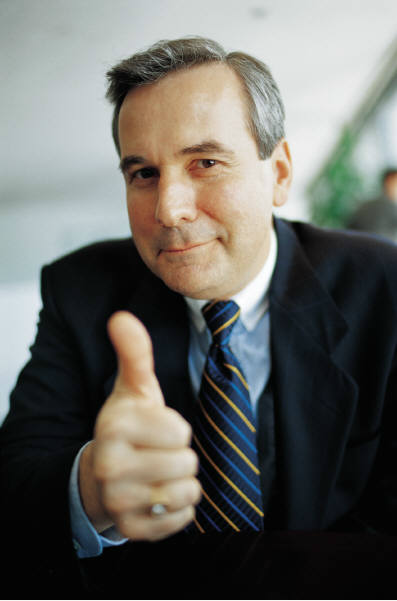
\includegraphics[width=0.7\textwidth]{boss.png}
\newpage
\tableofcontents


\end{center}
\end{titlepage}
\DeclareGraphicsExtensions{.jpg,~.pdf,~.mps,~.png,~.JPG}

%\author{KASIA JANOCHA, MICHAŁ PIEKARZ}
%\title{HAPPY BOSS
%\\CZYLI BĄDŹ ADMINEM WE WŁASNEJ FIRMIE}
%\date{}


%\begin{figure}[ht!]
%\centering
%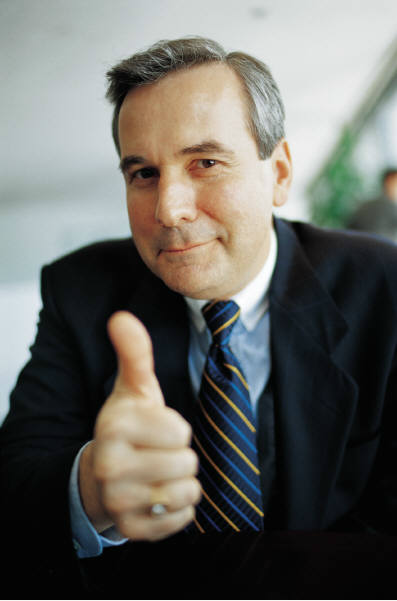
\includegraphics[width=90mm]{boss.png} 
%\label{overflow}
%\end{figure}

\section{Wstęp}

\begin{center}
\textit{Czyli o co chodzi w naszym projekcie?}
\end{center}

\subsection{Po co taki projekt?}

W dzisiejszych czasach młoda firma, która chce prężnie się rozwijać, często potrzebuje sieć komputerową na własne, wewnętrzne potrzeby.
Postanowiliśmy stworzyć aplikację, która pomoże rozwiązać ten problem.
Dzięki naszej aplikacji Użytkownik, który dokładnie i ze zrozumieniem przeczyta instrukcję, może samodzielnie zbudować prostą, ale niezwykle wydajną sieć komputerową na potrzeby swojej firmy.
\\\indent Ma to dla Użytkownika duże znaczenie - początkujące, młode firmy niekoniecznie mogą pozwolić sobie na zatrudnienie specjalisty.
\\\indent Dla ułatwienia Użytkownikowi pracy i zrozumienia działania aplikacji, wyposażyliśmy ją w dodatkową funkcjonalność - tworzenie wykresu sieci komputerowej. Dzięki niej Użytkownik pozna strukturę sieci, stanie się ona również niezwykłą pomocą w razie awarii sieci.

\subsection{Naukowe określenie problemu}

Tworzymy sieć komputerową o strukturze drzewowej, dla każdej maszyny istnieje z góry określona maksymalna pojemność - ilość maszyn, z którymi może być połączona (zakładamy, że jest to liczba większa od 2). Chcemy zachować najmniejszą możliwą średnicę sieci, tj. chcemy, aby odległość między najbardziej oddalonymi wierzchołkami była jak najmniejsza. Dochodzi nowy komputer, który musimy dodać on-line. Co robimy?


\section{Dokumentacja użytkowa}

\begin{center}
\textit{Czyli co użytkownik powinien wiedzieć}
\end{center}



\subsection{Czego użytkownik powinien oczekiwać?}
Prostej aplikacji, która pozwoli mu utworzyć własną sieć komputerową. Użytkownik powinien przygotować się na używanie linii komend.
Aplikacja, zainstalowana na danym komputerze, przyłączy komputer do sieci.

\subsection{Tworzenie wykresu}

\subsection{Jak uruchomić program?}

\subsection{Podsumowanie}
Jesteśmy pewni, iż dzięki powyższej instrukcji nawet Użytkownicy niezwiązani z branżą komputerową poradzą sobie z utworzeniem sieci komputerowej w swojej firmie!\\
Tych bardziej zorientowanych w temacie oraz ciekawych szczegółów technicznych zapraszamy do zapoznania się z dokumentacją implementacyjną oraz techniczną.

\section{Dokumentacja implementacyjna}

\begin{center}
\textit{Czyli szczegóły implementacyjne}
\end{center}



\subsection{Podstawowe dane na temat specyfikacji projektu}
WYBRANY JĘZYK: go\\
\\
POŁĄCZENIE MIĘDZY KOMUPUTERAMI: socket\\
\\
POZOSTAŁE TECHNOLOGIE: Google Charts (https://developers.google.com/chart/)\\
\\

\subsection{Podstawowe dane na temat specyfikacji projektu}


\section{Dokumentacja techniczna}

\begin{center}
\textit{Czyli szczegóły techniczne}
\end{center}

\subsection{Klient - serwer}
Podstawową jednostką naszej sieci jest klient, czyli użytkownik. Klientem takim jest nowo dołączany komputer. Najważniejszą funkcjonalnością sieci jest komunikacja klienta z serwerem.\\
\indent Za obsługę tejże komunikacji odpowiedzialny jest package joinservice, a konkretnie - znajdujące się w nim implementacje client.go i server.go.\\
\indent Techniczne szczegóły dotyczące zamieszczonych w nich konstruktorów i metod znnajdują się w komentarzach, a zatem również w wygenerowanym docu. Komentarze są na tyle dokładne, ze nie wymagają dodatkowego tłumaczenia - zapraszamy do ich lektury!

\subsection{Drzewo}
Funkcjonalności naszej sieci opierają się na strukturze drzewa, które tworzy. Odpowiada za nie joinservice/tree.\\
\indent Klasa node.go trzyma reprezentację drzewa jako drzewa wskaźnikowego - każdy wierzchołek ma listę wskaźników do swoich dzieci.\\
\indent Funkcje DFS oraz FindSolution przeszukują drzewo metodą DFS na potrzeby obu funkcjonalności, które oferujemy.\\
\indent Dlatego obsługę drzewa zdecydowaliśmy się umieścić w pakiecie z klientem i serwerem. Jest to klasa kluczowa dla działania całej algorytmiki w aplikacji.

\subsection{Protokoły}
...znajdują się w pakiecie protocols. Opis ich działania zamieściliśmy w dokumentacji implementacyjnej.\\
\indent Z kodu w oczywisty sposób wynikają uzasadnienia poszczególnych naszych decyzji.\\
\indent Funkcje znajdujące się w protokołach to głównie funkcje pomocnicze służące do interpretacji, parse'owania i obsługi danych.\\
\indent Za budowę wiadomości odpowiada struct Message (w każdym protokole z osobna). W przypadku STP jest niezwykle prosty. Sposób, w jaki używamy go w SIP jasno wynika z komentarzy. Są w nich wyszczególnione możliwe typy wiadomości - są one kluczowe w naszej aplikacji, warto się z nimi zapoznać!

\subsection{Pakiet resources}
\indent odpowiada za skrypt tworzenia grafu. Jest w niego wpisany kod skryptu, komputery budują odpowiedni plik łącząc pliki odpowiadające za początek i koniec skryptu.\\
\indent Zdecydowaliśmy się na takie rozwiązanie, ponieważ musimy wpisać "środek skryptu", który jest zmienny i odpowiada za kształt wykresu (patrz klasa node.go - jego funkcja DFS wpisuje do odpowiedniego pliku tenże "środek").

\subsection{Szczegółowy opis działania wszystkich funkcji}
...znajduje się w anglojęzycznym docu: \url{http://godoc.org/github.com/pitex/sieci-projekt/src}\\
\indent Opisy są bardzo dokładne - zapraszamy do lektury!


\section{Podział pracy}

\begin{center}
\textit{Co kto robił?}
\end{center}

\subsection{Słowo wstępu}
Większa część projektu była pracą wspólną, dlatego w niektórych momentach ciężko jest wyodrębnić role poszczególnych członków zespołu. Większość czasu spędzonego nad projektem to dyskusje i projektowanie - w tym oboje mieliśmy równy udział. Dlatego też postanowiliśmy podzielić poszczególne zadania na robione wspólnie i te, którymi zajmowała się głównie jedna osoba.


\subsection{Część, nad którą pracowaliśmy wspólnie}
\begin{enumerate}
\item % 1
Ogólny projekt aplikacji;
\item % 2
Ogólny projekt protokołów;
\item % 3
Szczegółowa implementacja serwera.
\end{enumerate}


\subsection{Michał}
\begin{enumerate}
\item % 1
Ogólny projekt i implementacja schematu protokołów;
\item % 2
Implementacja schematu klient-server;
\item % 3
Testowanie;
\item % 4
Większość debugu.

\end{enumerate}


\subsection{Kasia}
\begin{enumerate}
\item % 1
Większość funkcji pomocniczych protokołu SIP;
\item % 2
Budowanie drzewa, implementacja node;
\item % 3
Część związana z obsługą Google Charts i ogólną budową wykresu;
\item % 4
Algorytmika dodawania nowego węzła sieci.

\end{enumerate}

\end{document}
